% !TEX program = pdflatex
% Boson14 Planted-Clique Benchmark — Variant & Amplitude Sweep
% Compile: pdflatex report.tex (run twice for correct references)

\documentclass[aspectratio=169]{beamer}
\usetheme{metropolis}

\usepackage{amsmath,amssymb}
\usepackage{booktabs}
\usepackage{listings}
\usepackage{xcolor}
\usepackage{graphicx}
\usepackage{hyperref}

% Figure path so \includegraphics can find PNGs by short name.
\graphicspath{{figures/}}

% Metadata
\title{Boson14 Planted-Clique Benchmark}
\subtitle{Variant \& Amplitude Sweep on Motzkin--Straus StQP}
\author{QCi Hardware Team}
\date{\today}
\institute{Quantum Computing Inc.}

\begin{document}

% ── Title ─────────────────────────────────────────────────────────────────

\maketitle

% ── Motzkin--Straus recap ─────────────────────────────────────────────────

\begin{frame}{Motzkin--Straus in the scaled simplex}
Given an undirected graph $G=(V,E)$ with adjacency $A$, the \emph{standard
quadratic program} over the scaled simplex is
\[
\max_{y \ge 0,\; \sum_i y_i = R}\; g(y) \;=\; \tfrac{1}{2}\, y^\top A\, y .
\]
The Motzkin--Straus theorem gives the optimum as a function of the clique number $\omega$:
\[
g^\ast(\omega) \;=\; \frac{R^{2}}{2}\!\left(1 - \frac{1}{\omega}\right),
\qquad
\omega \;=\; \operatorname{round}\!\left(\frac{R^{2}}{R^{2} - 2\, g^\ast}\right).
\]
Boson14 maximises $y^\top A\, y = 2\,g(y)$ under the sum constraint $R$, so the
relation between the reported hardware ``energy'' and the scaled objective is
\[
\texttt{energy\_list}[i] \;=\; y_i^\top A\, y_i \;=\; 2\, g(y_i).
\]
\end{frame}

% ── Experimental design ───────────────────────────────────────────────────

\begin{frame}{Experimental design}
\begin{columns}[T]
\begin{column}{0.58\textwidth}
Six planted-clique StQP instances; for each, the clique is placed at three
different matrix positions and each placement is submitted at four boson14
amplitudes.
\begin{itemize}
  \item \textbf{Variants} (index scrambling):
    \textit{random} (original), \textit{front} (clique at indices $1..k$),
    \textit{end} (indices $n{-}k{+}1..n$).
  \item \textbf{Amplitudes}: $a \in \{300, 400, 500, 600\}$
        (one instance uses $a=380$ and another adds $a=700$).
  \item \textbf{Samples per run}: 100. Sum constraint $R=100$.
\end{itemize}
\end{column}
\begin{column}{0.42\textwidth}
\scriptsize
\begin{tabular}{@{}lrrrr@{}}
\toprule
instance & $n$ & $k$ & $p$ & $g^*$ \\
\midrule
n20\_k5   & 20  & 5  & 0.3 & 4000.0 \\
n20\_k6   & 20  & 6  & 0.2 & 4166.7 \\
n50\_k10  & 50  & 10 & 0.3 & 4500.0 \\
n50\_k22  & 50  & 22 & 0.5 & 4772.7 \\
n100\_k22 & 100 & 22 & 0.2 & 4772.7 \\
n100\_k63 & 100 & 63 & 0.7 & 4920.6 \\
\bottomrule
\end{tabular}
\vskip 4pt
\tiny Seed $= 42$, $R = 100$ for all instances.
\end{column}
\end{columns}
\end{frame}

% ── Test graphs (3 frames, grouped by size) ───────────────────────────────

\begin{frame}{Test graphs: $n=20$ (planted clique highlighted)}
\centering

\includegraphics[height=0.80\textheight]{graphs/benchmark_n20_k5_p0.3_s42.png}\hfill

\includegraphics[height=0.80\textheight]{graphs/benchmark_n20_k6_p0.2_s42.png}\\
\footnotesize Red nodes = planted maximum clique (brute-force verified $\omega=k$).
\end{frame}

\begin{frame}{Test graphs: $n=50$ (planted clique highlighted)}
\centering

\includegraphics[height=0.80\textheight]{graphs/benchmark_n50_k10_p0.3_s42.png}\hfill

\includegraphics[height=0.80\textheight]{graphs/benchmark_n50_k22_p0.5_s42.png}\\
\footnotesize Inner ring = clique nodes, outer ring = remaining vertices.
\end{frame}

\begin{frame}{Test graphs: $n=100$ (planted clique highlighted)}
\centering

\includegraphics[height=0.80\textheight]{graphs/benchmark_n100_k22_p0.2_s42.png}\hfill

\includegraphics[height=0.80\textheight]{graphs/benchmark_n100_k63_p0.7_s42.png}\\
\footnotesize Clique-only labels shown to keep the figure legible at $n=100$.
\end{frame}

% ── Per-instance results (6 frames, one per instance) ─────────────────────

\begin{frame}{Results: \texttt{n20\_k5} ($k=5$, $g^\ast=4000$)}
\centering
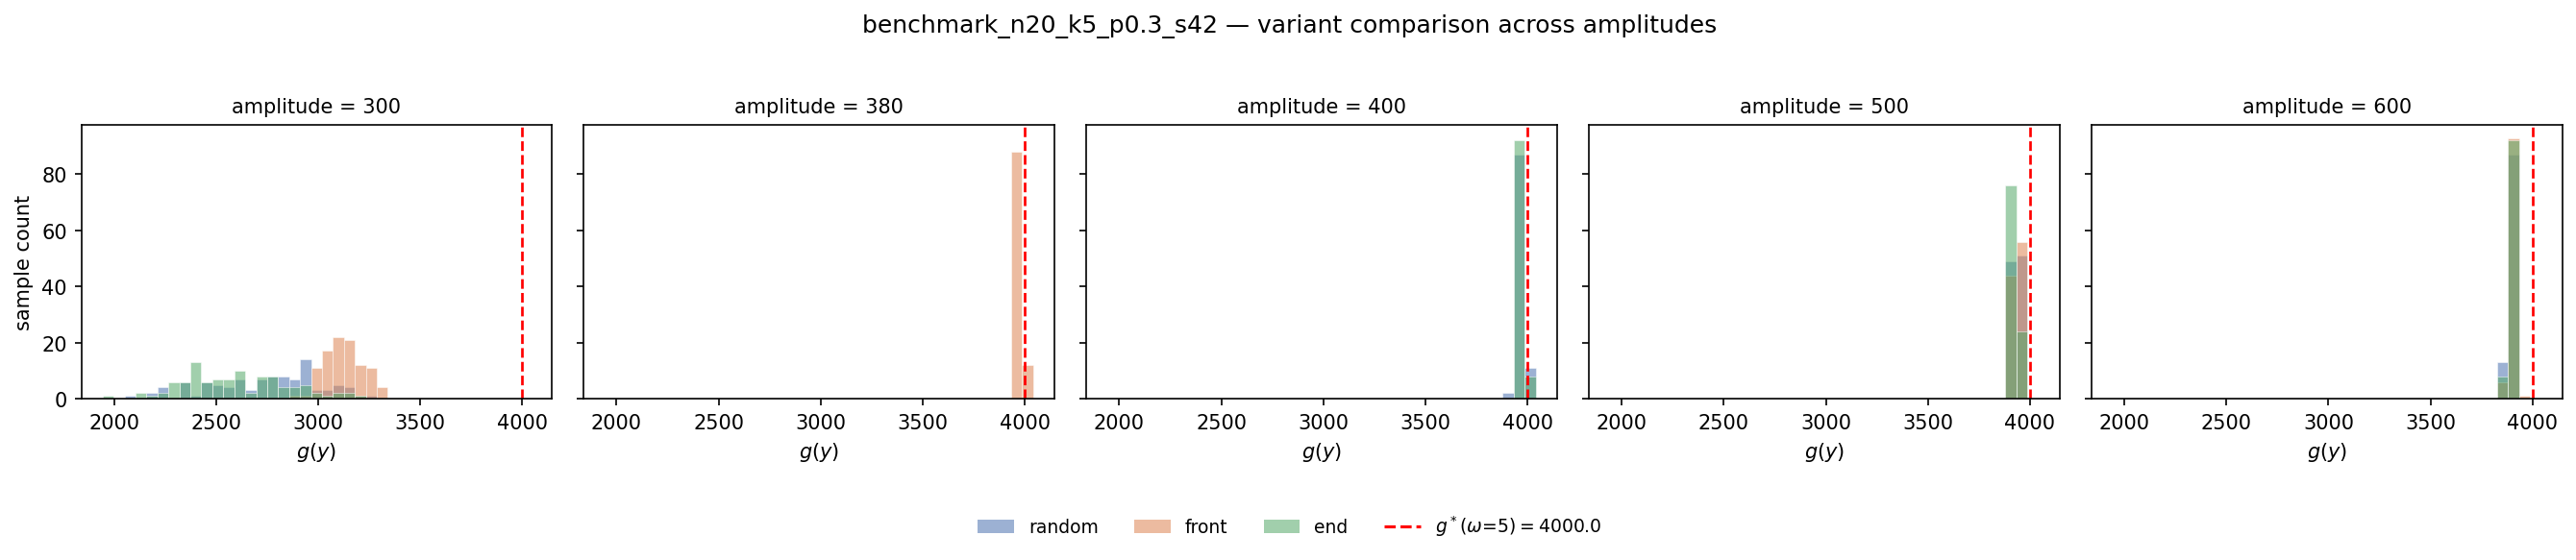
\includegraphics[width=0.95\linewidth]{benchmark_n20_k5_p0.3_s42/hist_overlay_benchmark_n20_k5_p0.3_s42.png}\\
\footnotesize
Best sample hits $99.93\%$ of $g^\ast$ (front, $a=380$); omega-hit rate
reaches $100\%$ at $a\in\{400,500\}$. Variants overlap almost perfectly.
\end{frame}

\begin{frame}{Results: \texttt{n20\_k6} ($k=6$, $g^\ast=4167$)}
\centering
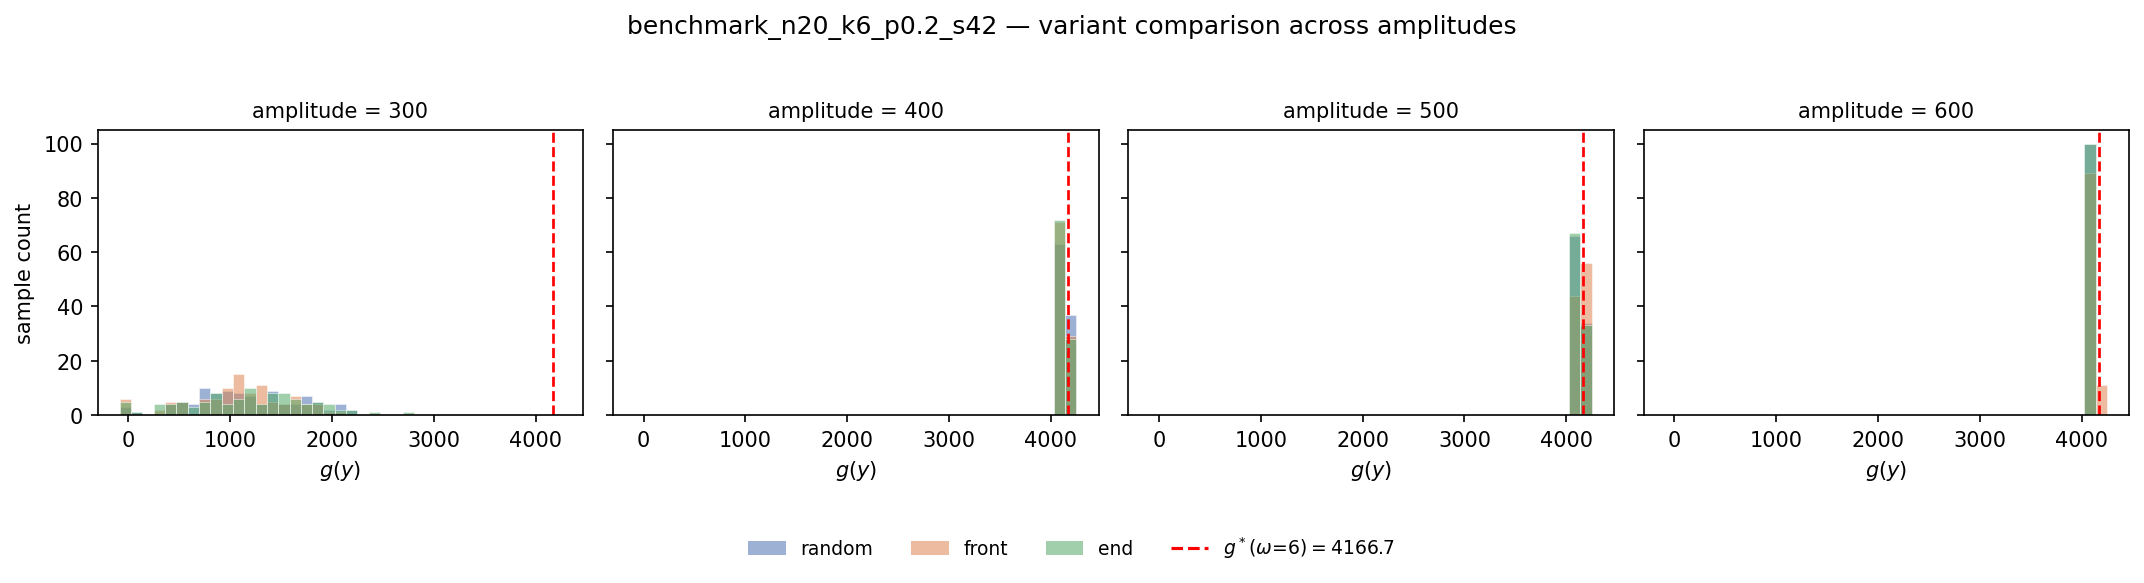
\includegraphics[width=0.95\linewidth]{benchmark_n20_k6_p0.2_s42/hist_overlay_benchmark_n20_k6_p0.2_s42.png}\\
\footnotesize
Best sample hits $99.95\%$ of $g^\ast$ (front, $a=500$); omega-hit rate
peaks at $100\%$ for all variants at $a=500$, drops at $a=600$.
\end{frame}

\begin{frame}{Results: \texttt{n50\_k10} ($k=10$, $g^\ast=4500$)}
\centering
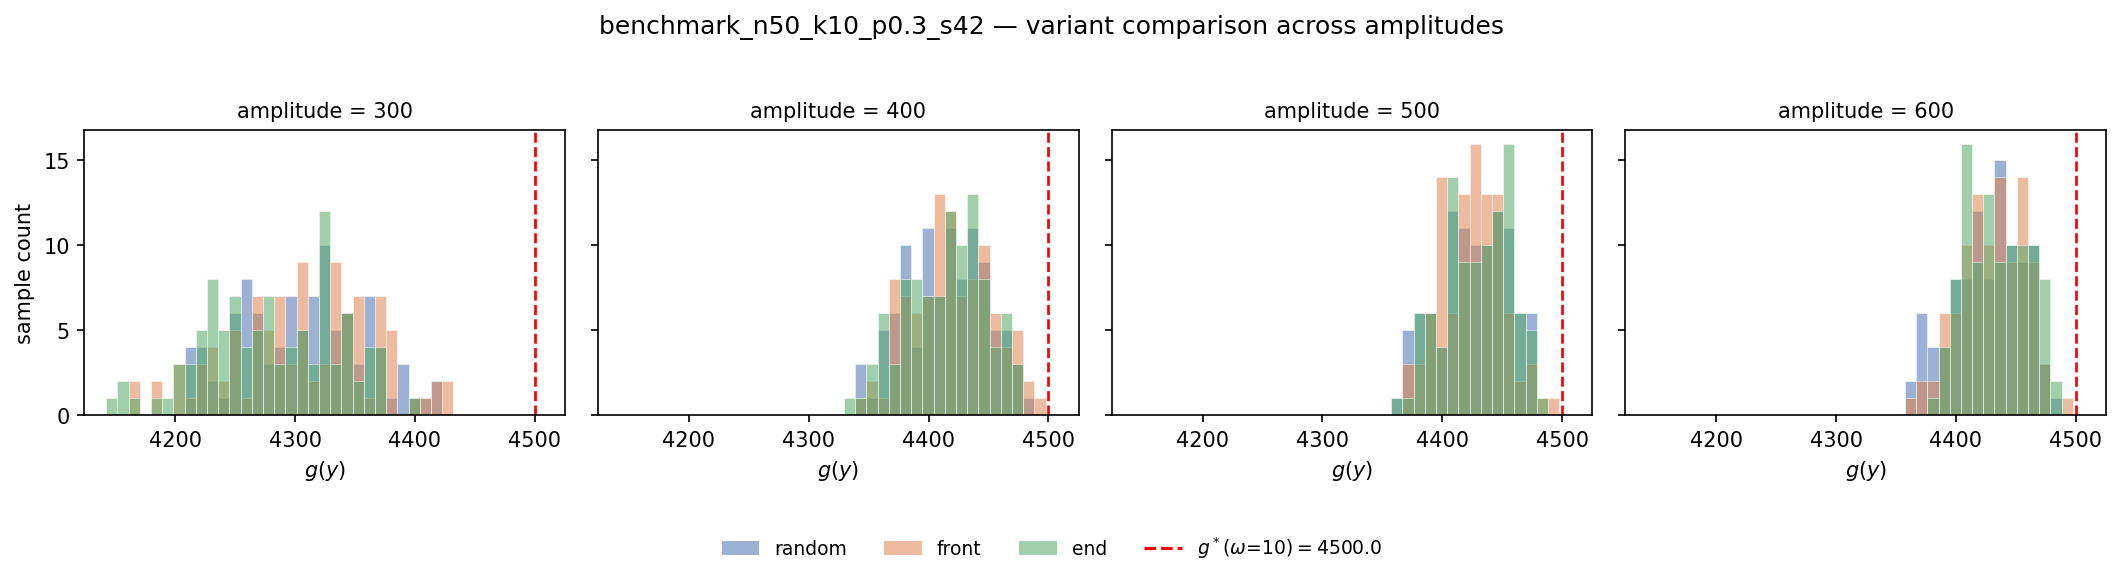
\includegraphics[width=0.95\linewidth]{benchmark_n50_k10_p0.3_s42/hist_overlay_benchmark_n50_k10_p0.3_s42.png}\\
\footnotesize
Best sample hits $99.86\%$ of $g^\ast$ (front, $a=500$). Distributions now
concentrate just below $g^\ast$; omega-hit rate collapses to $\le 7\%$
despite the gap being under $0.3\%$.
\end{frame}

\begin{frame}{Results: \texttt{n50\_k22} ($k=22$, $g^\ast=4773$)}
\centering
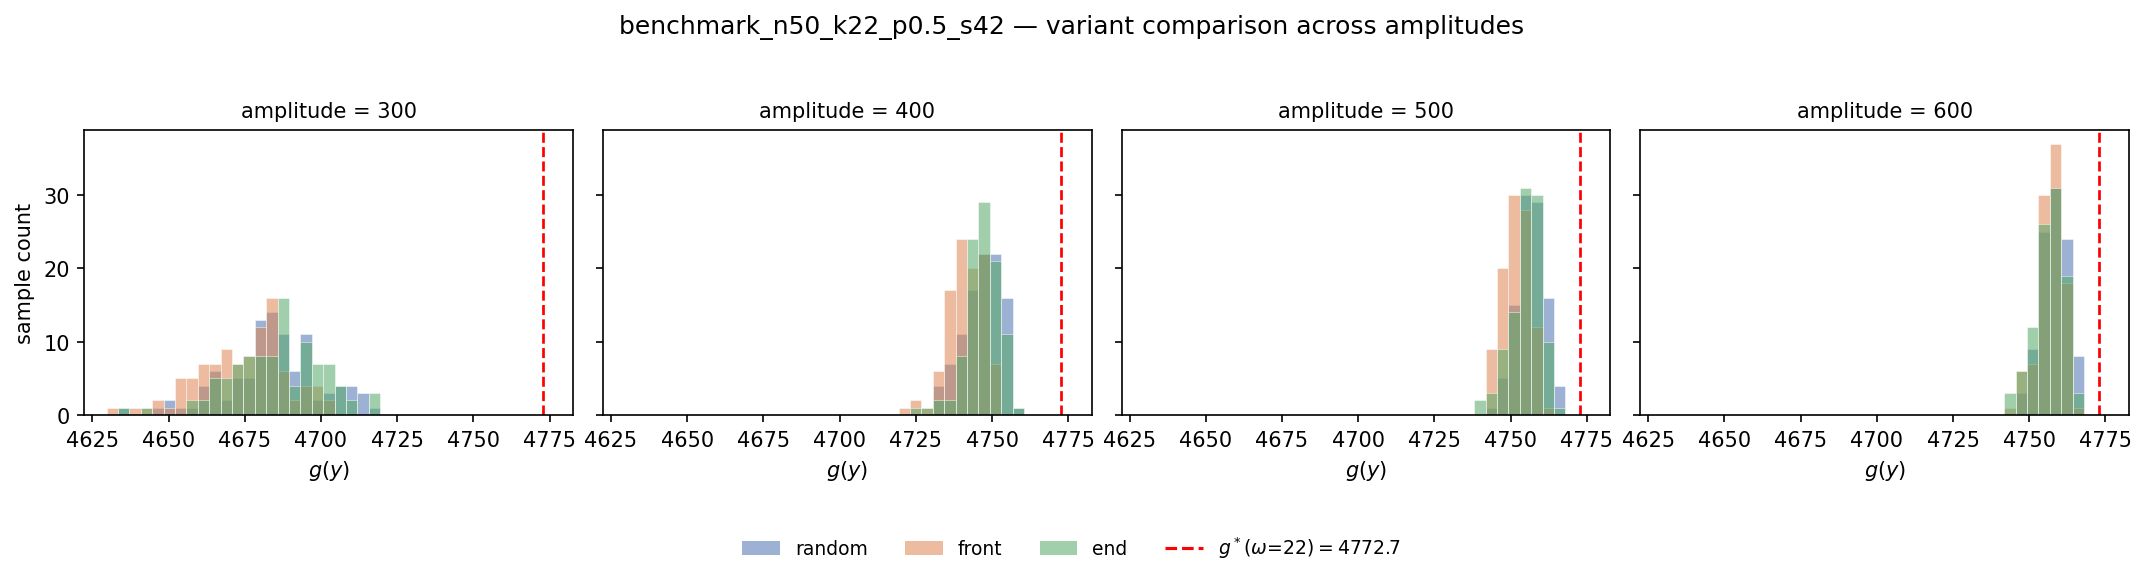
\includegraphics[width=0.95\linewidth]{benchmark_n50_k22_p0.5_s42/hist_overlay_benchmark_n50_k22_p0.5_s42.png}\\
\footnotesize
Best sample hits $99.88\%$ of $g^\ast$ (random, $a=600$). Omega rounding
never lands exactly at $k=22$ — integer recovery fails at this resolution.
\end{frame}

\begin{frame}{Results: \texttt{n100\_k22} ($k=22$, $g^\ast=4773$)}
\centering
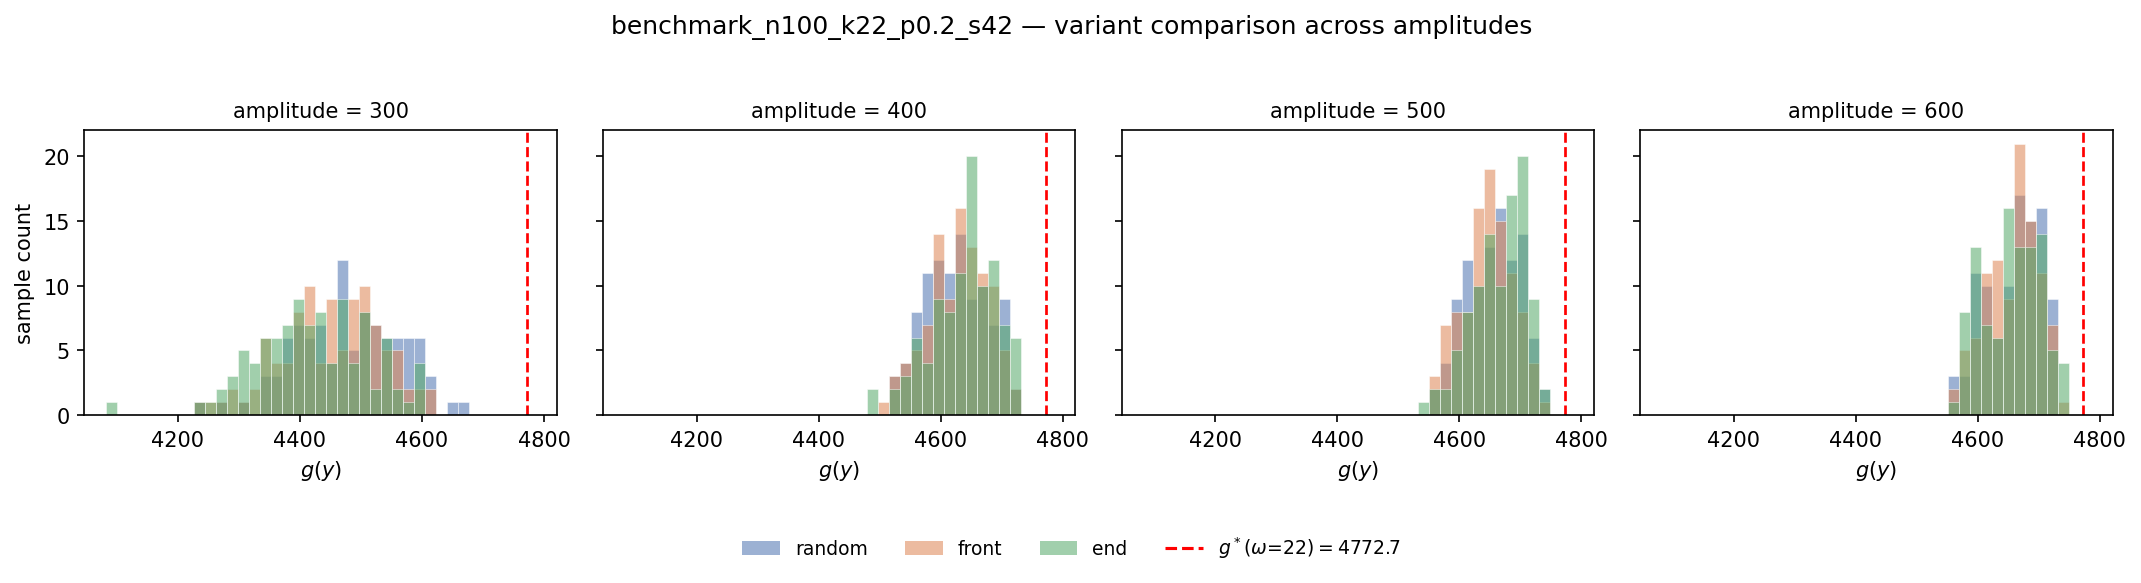
\includegraphics[width=0.95\linewidth]{benchmark_n100_k22_p0.2_s42/hist_overlay_benchmark_n100_k22_p0.2_s42.png}\\
\footnotesize
Best sample hits $99.41\%$ of $g^\ast$ (front, $a=600$). Larger $n$ shifts
the entire distribution slightly further below the MS line.
\end{frame}

\begin{frame}{Results: \texttt{n100\_k63} ($k=63$, $g^\ast=4921$)}
\centering
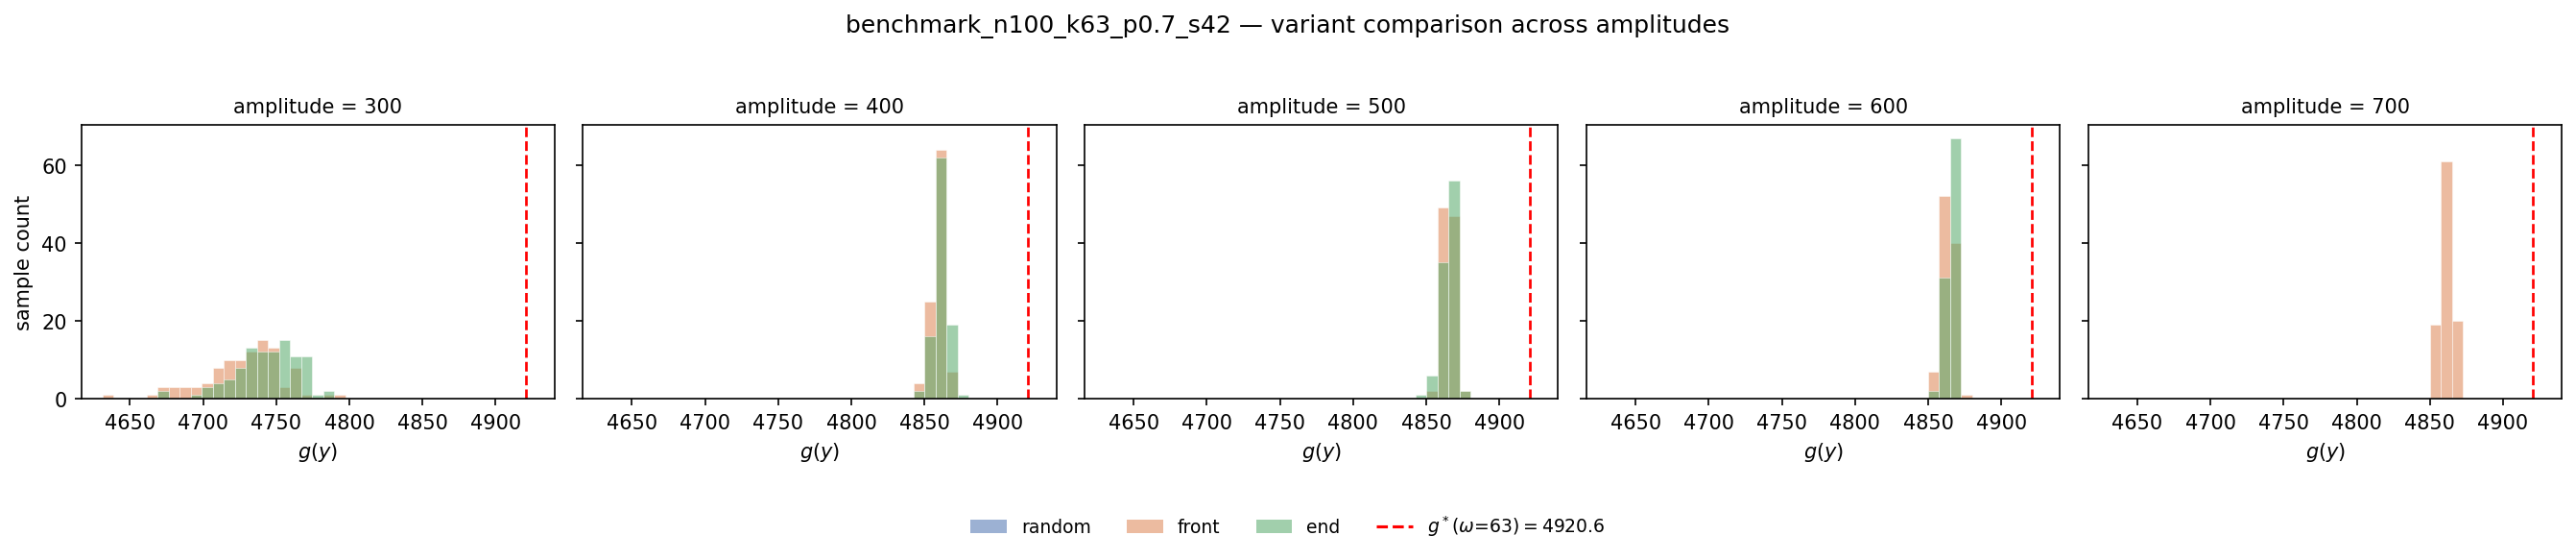
\includegraphics[width=0.95\linewidth]{benchmark_n100_k63_p0.7_s42/hist_overlay_benchmark_n100_k63_p0.7_s42.png}\\
\footnotesize
Densest graph ($p=0.7$). Best sample hits $99.06\%$ of $g^\ast$ (end,
$a=400$). \textit{Random} variant missing — only \textit{front}/\textit{end}
were submitted for this instance; \textit{front} has an extra $a=700$ run.
\end{frame}

% ── Dirac-3 comparison (3 frames, grouped by size) ────────────────────────

\begin{frame}{Dirac-3 vs boson14 ($a{=}600$): $n=20$}
\centering
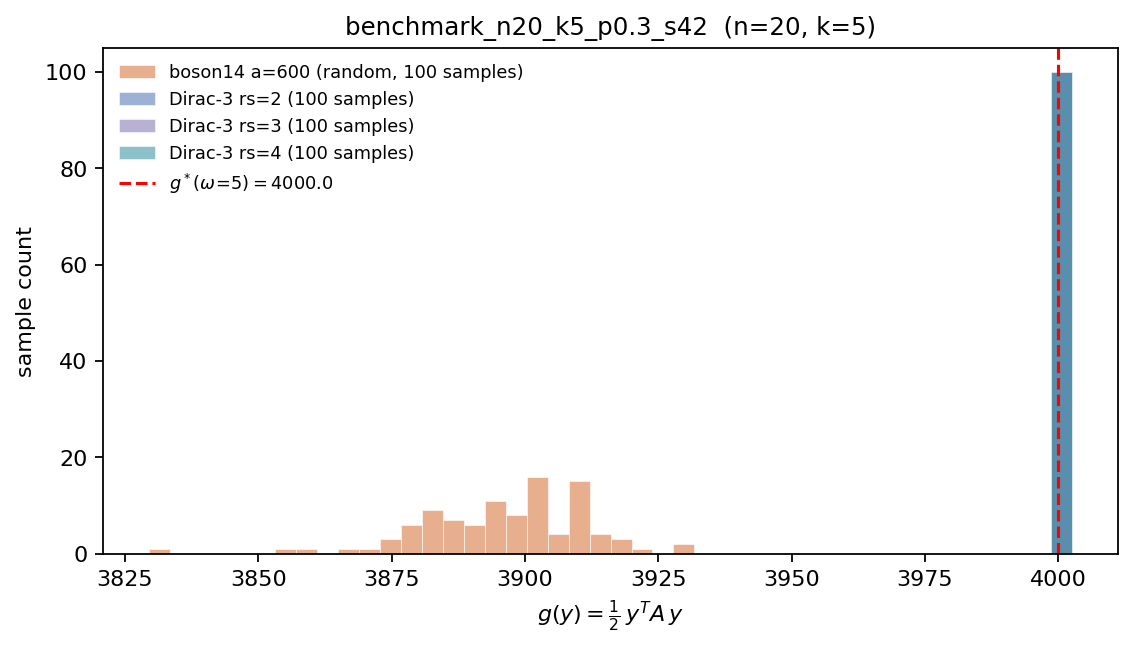
\includegraphics[width=0.49\linewidth]{dirac_overlay/benchmark_n20_k5_p0.3_s42.png}\hfill
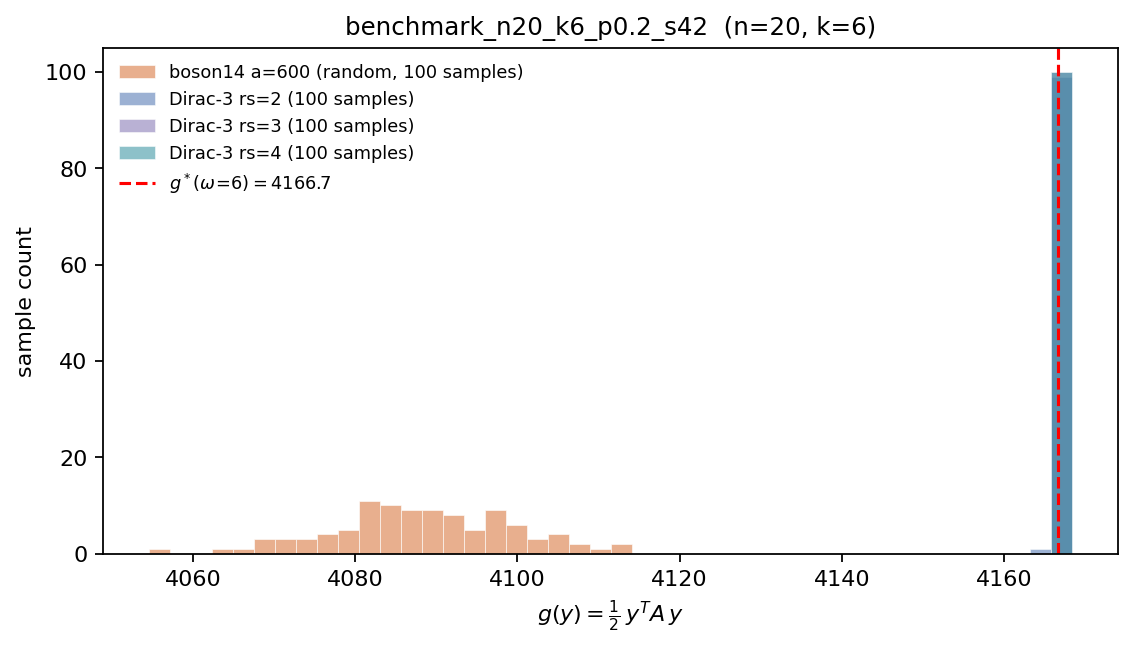
\includegraphics[width=0.49\linewidth]{dirac_overlay/benchmark_n20_k6_p0.2_s42.png}\\
\footnotesize
Each Dirac run: 100 samples at relaxation-schedule $\in\{2,3,4\}$. On small
graphs Dirac-3 locks onto $g^\ast$; boson14 at its best amplitude still
sits a few percent below.
\end{frame}

\begin{frame}{Dirac-3 vs boson14 ($a{=}600$): $n=50$}
\centering
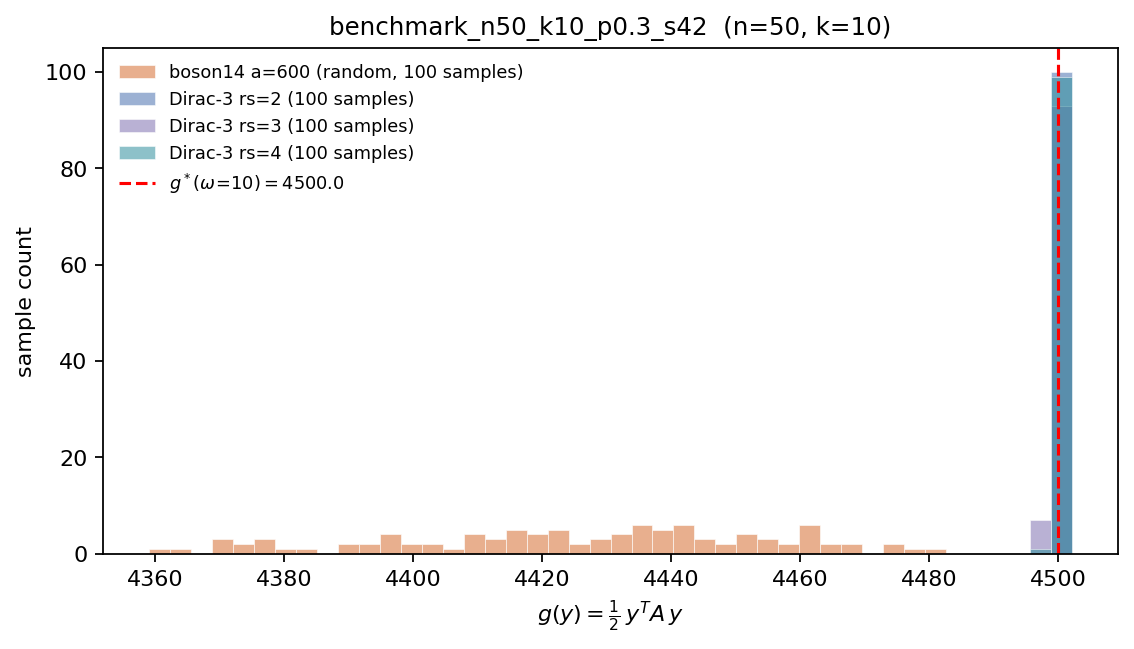
\includegraphics[width=0.49\linewidth]{dirac_overlay/benchmark_n50_k10_p0.3_s42.png}\hfill
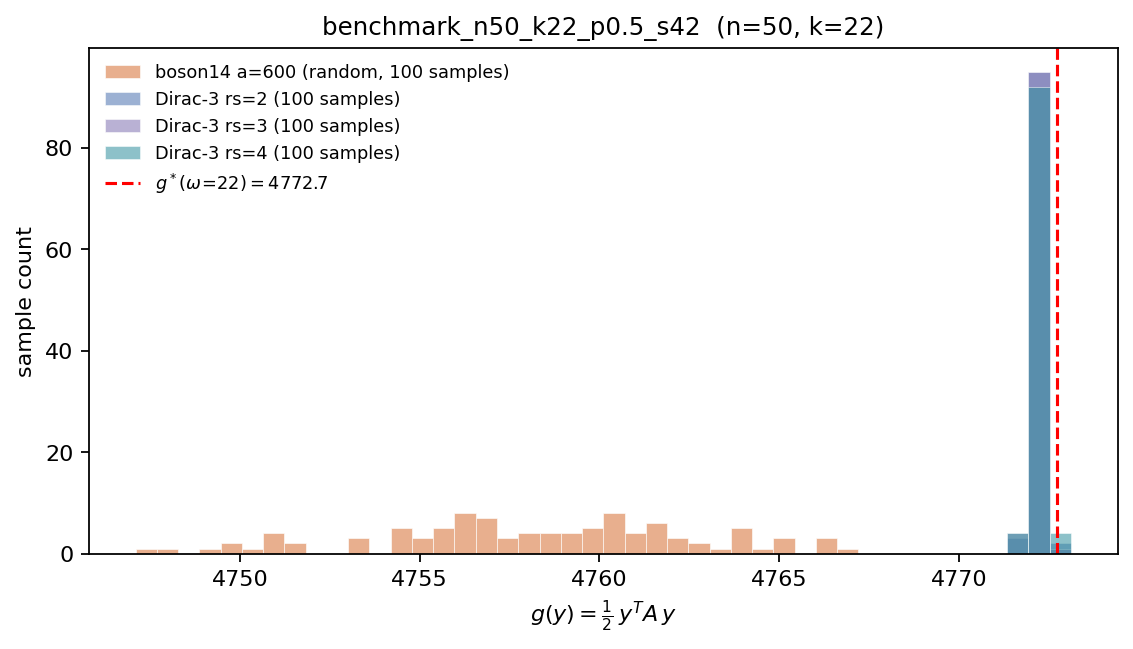
\includegraphics[width=0.49\linewidth]{dirac_overlay/benchmark_n50_k22_p0.5_s42.png}\\
\footnotesize
Dirac-3 and boson14 become more comparable as $n$ grows. Schedule effect
on Dirac is small; both solvers sample within a narrow band below $g^\ast$.
\end{frame}

\begin{frame}{Dirac-3 vs boson14 ($a{=}600$): $n=100$}
\centering
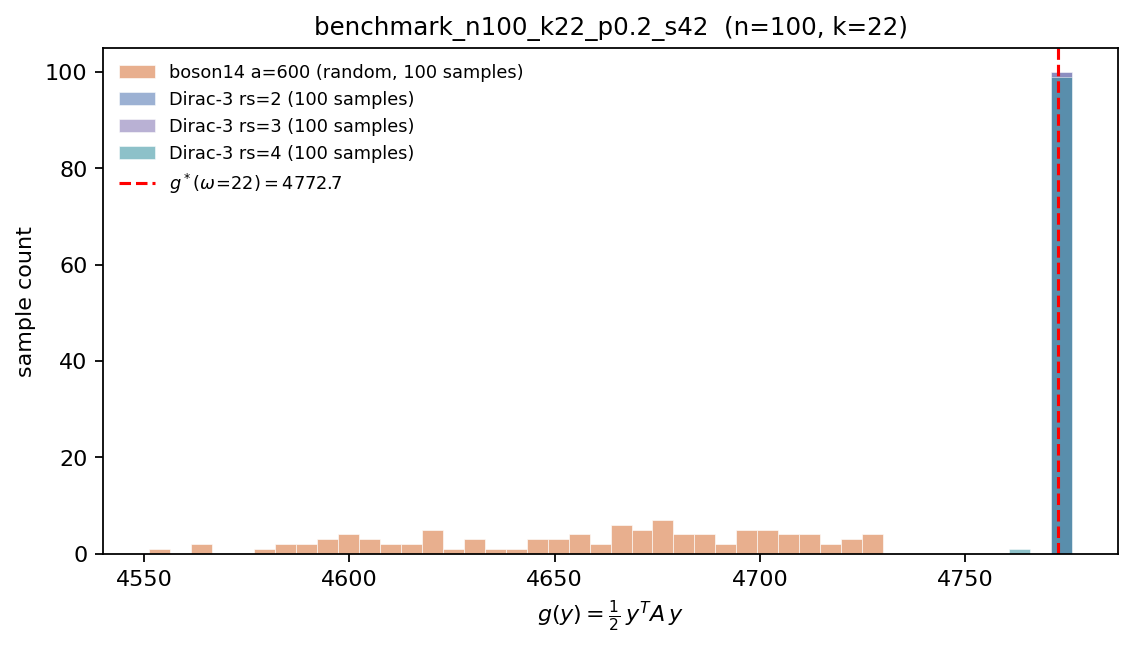
\includegraphics[width=0.49\linewidth]{dirac_overlay/benchmark_n100_k22_p0.2_s42.png}\hfill
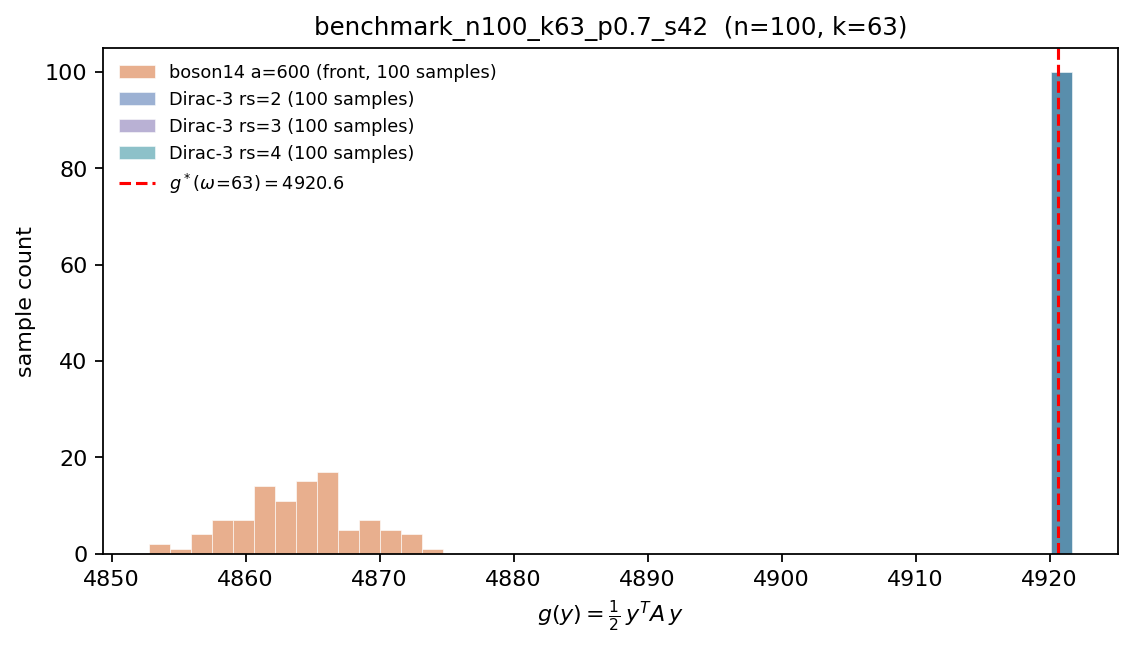
\includegraphics[width=0.49\linewidth]{dirac_overlay/benchmark_n100_k63_p0.7_s42.png}\\
\footnotesize
Largest instances. Dirac-3 rs=4 gives the tightest high-$g$ cluster; boson14
$a=600$ histogram is comparable in spread but offset. MS line at $g^\ast$.
\end{frame}

% ── Dirac sanity check ───────────────────────────────────────────────────

\begin{frame}{Sanity check: do Dirac-3 solutions correspond to real cliques?}
\footnotesize
For each of the 18 runs, take the best sample $y$, threshold the support at
$y_i > R/(2k)$, and verify: \textbf{(i)} $|S|=\omega$, \textbf{(ii)} every
pair in $S$ is an edge of $G$, \textbf{(iii)} $y_i \approx R/\omega$ on $S$.
\vskip 3pt
\centering
\renewcommand{\arraystretch}{1.05}
\begin{tabular}{@{}lccccc@{}}
\toprule
instance & rs & $|S|$ & clique? & matches planted & $y_{S}$ mean\,$\pm$\,std (ideal $R/\omega$) \\
\midrule
n20\_k5   & 2/3/4 & 5/5 & \checkmark & \textit{alt clique} & $18.8\pm 2.3$ (20.0) \\
n20\_k6   & 2/3/4 & 6/6 & \checkmark & yes & $16.67\pm 0.09$ (16.67) \\
n50\_k10  & 2/3/4 & 10/10 & \checkmark & yes & $10.00\pm 0.15$ (10.00) \\
n50\_k22  & 2/3/4 & 22/22 & \checkmark & yes & $\phantom{0}4.545\pm 0.12$ (4.545) \\
n100\_k22 & 2/3/4 & 22/22 & \checkmark & yes & $\phantom{0}4.545\pm 0.09$ (4.545) \\
n100\_k63 & 2/3/4 & 63/63 & \checkmark & yes & $\phantom{0}1.587\pm 0.04$ (1.587) \\
\bottomrule
\end{tabular}
\vskip 4pt
\footnotesize
\textbf{All 18 supports are valid max cliques.} The \emph{n20\_k5} graph
happens to contain 4 distinct 5-cliques; Dirac consistently landed on
$\{2,3,9,12,14\}$ instead of the planted $\{2,9,12,14,20\}$ — both have
$|S|=\omega=5$, so MS objective is indifferent. The wider std on its
support reflects proximity to a convex combination of overlapping optima.
\end{frame}

% ── boson14 post-processing: repair analysis ─────────────────────────────

\begin{frame}{Repairing boson14 samples}
\footnotesize
Apply the same threshold $y_i > R/(2k)$ to every boson14 sample to
extract a support $S$.  Three derived quantities per sample:
\begin{itemize}
  \item \textbf{raw} — $g(y) = \tfrac12 y^\top A y$ on the continuous vector;
  \item \textbf{equal-weight} — when $S$ is a clique, the MS-optimal
        embedding on it has $g=\tfrac{R^2}{2}(1-1/|S|)$;
  \item \textbf{1-opt repaired} — seed the support, iteratively remove the
        worst-connected vertex until $S$ is a clique, then greedily add any
        vertex adjacent to all of $S$ until maximal. Report equal-weight $g$.
\end{itemize}
Aggregate over all 6\,900 boson14 samples (6 graphs $\times$ 3 variants
$\times$ up to 4 amplitudes $\times$ 100):
\vskip 2pt
\centering
\begin{tabular}{@{}lrr@{}}
\toprule
& runs (of 69) & samples (of 6\,900) \\
\midrule
Threshold-support is itself a clique       & 57 runs 100\%      & 6\,477 / 6\,900 (93.9\%) \\
1-opt repair reaches exactly $\omega$      & 65 runs 100\%      & 6\,527 / 6\,900 (94.6\%) \\
1-opt reaches $\omega$ at $a=600$ only     & \textbf{all 17}    & \textbf{1\,700 / 1\,700 (100\%)} \\
\bottomrule
\end{tabular}
\vskip 3pt
\footnotesize
At $a=600$ (best amplitude), 1-opt recovers $\omega$ for \textbf{every
single sample on every graph}. The failures are concentrated at $a=300$
where the continuous output has too little mass on the right vertices for
greedy extension to find them.
\end{frame}

\begin{frame}{Repair overlays: $n=20$}
\centering

\includegraphics[width=0.49\linewidth]{repair/benchmark_n20_k5_p0.3_s42.png}\hfill

\includegraphics[width=0.49\linewidth]{repair/benchmark_n20_k6_p0.2_s42.png}\\
\footnotesize
Orange: raw boson14 at $a=600$.  Blue: equal-weight MS value on samples
whose threshold-support is already a clique.  Faint red outline at
$g^\ast$: all 100 samples after 1-opt repair.
\end{frame}

\begin{frame}{Repair overlays: $n=50$}
\centering

\includegraphics[width=0.49\linewidth]{repair/benchmark_n50_k10_p0.3_s42.png}\hfill

\includegraphics[width=0.49\linewidth]{repair/benchmark_n50_k22_p0.5_s42.png}\\
\footnotesize
Raw boson14 sits a few percent below $g^\ast$; 1-opt moves \emph{every}
sample to the MS optimum. On \texttt{n50\_k10} the threshold-support is
already size-$k$ and valid in all 100 samples.
\end{frame}

\begin{frame}{Repair overlays: $n=100$}
\centering

\includegraphics[width=0.49\linewidth]{repair/benchmark_n100_k22_p0.2_s42.png}\hfill

\includegraphics[width=0.49\linewidth]{repair/benchmark_n100_k63_p0.7_s42.png}\\
\footnotesize
Largest graphs. The repair gap (raw $\to g^\ast$) is visually dramatic on
\texttt{n100\_k63}, but 1-opt still recovers the full $63$-clique in every
sample. The continuous output contains enough structural information even
when the raw $g$ is 1\% below optimal.
\end{frame}

% ── Aggregate view ────────────────────────────────────────────────────────

\begin{frame}{Aggregate: success rate and best-sample closeness}
\begin{columns}[T]
\begin{column}{0.52\textwidth}
\centering
\footnotesize fraction of 100 samples with $\omega_{\mathrm{est}} \ge k$\\
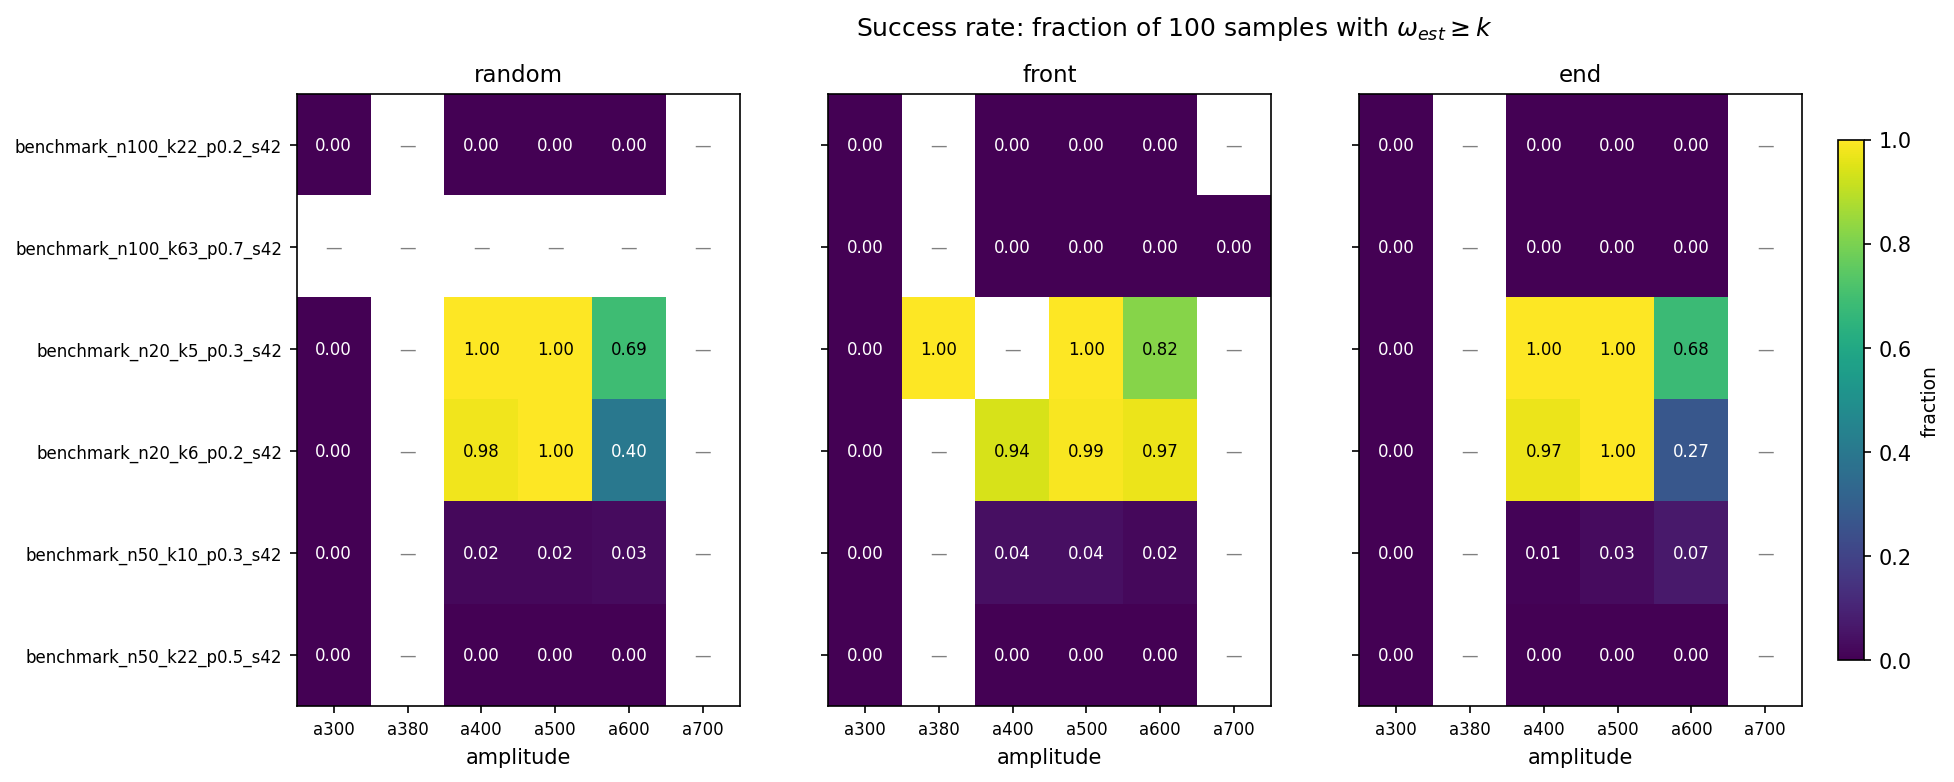
\includegraphics[width=\linewidth]{summary_success_rate.png}
\end{column}
\begin{column}{0.48\textwidth}
\centering
\footnotesize $g_{\mathrm{best}} / g^\ast$ \hspace{4pt}(scale $0.9$--$1.0$)\\
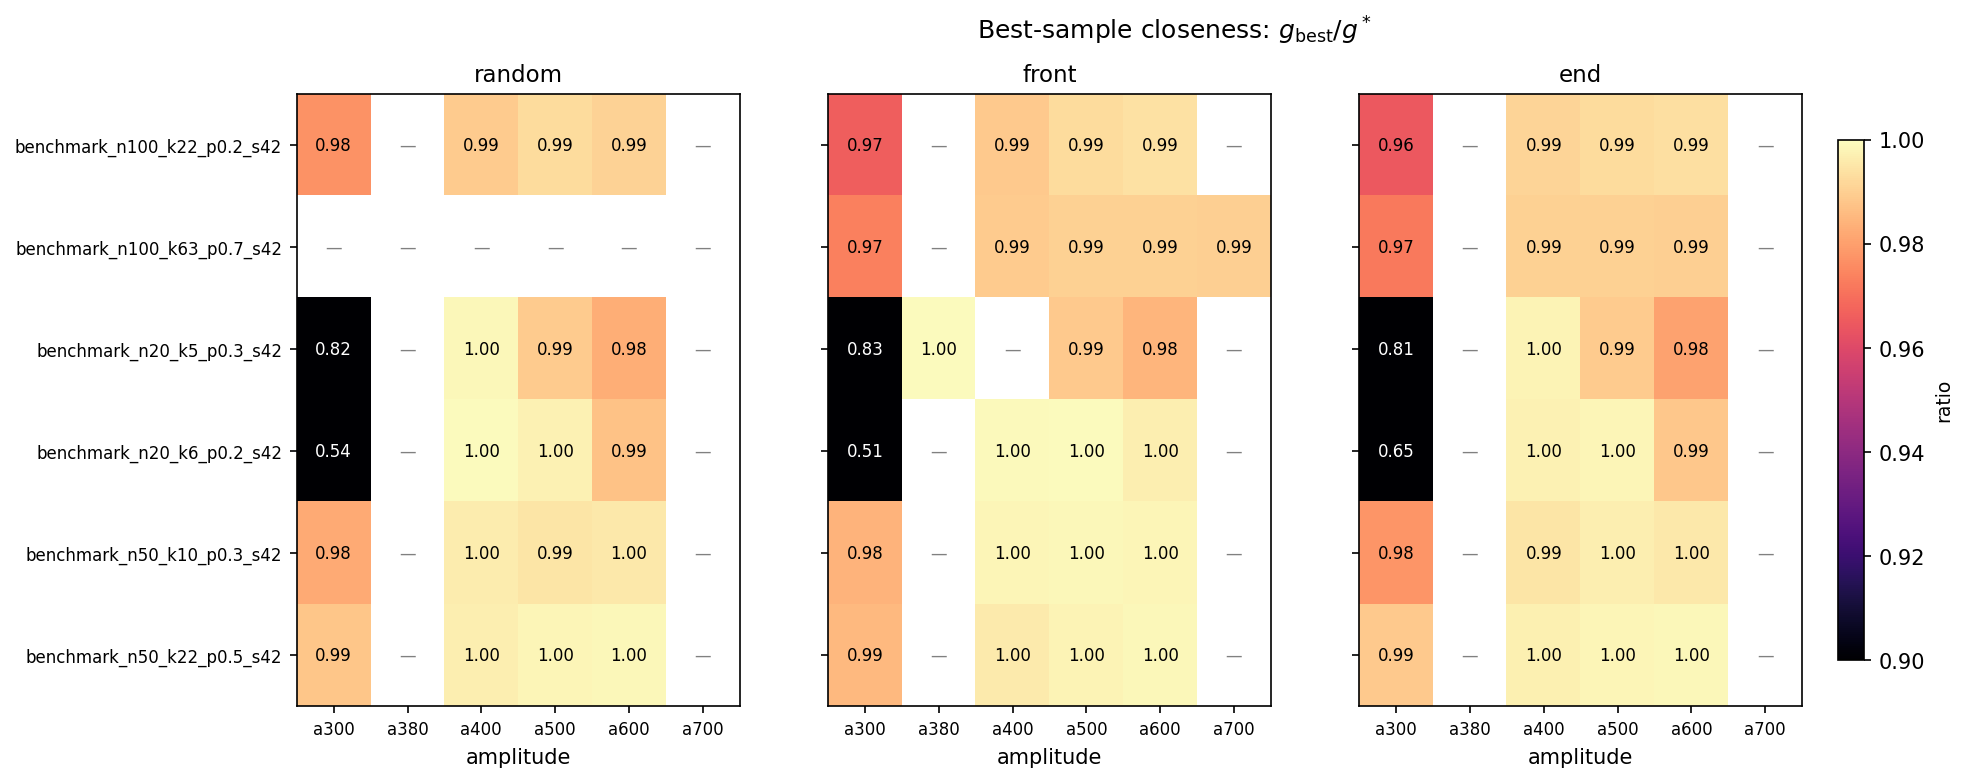
\includegraphics[width=\linewidth]{summary_best_ratio.png}
\end{column}
\end{columns}
\vskip 4pt
\footnotesize
Left: exact omega recovery is reliable only for $k\!\le\!6$. Right: boson14
reaches $\ge 99\%$ of $g^\ast$ on \emph{every} amplitude except $a=300$, where
small-$n$ runs fail to converge ($0.51$--$0.83$).
\end{frame}

% ── Discussion ────────────────────────────────────────────────────────────

\begin{frame}{Findings}
\begin{itemize}
  \item \textbf{Clique-index permutation does not affect performance.}
        Across all instances the best $g$ across variants differs by at most
        $\mathbf{0.24\%}$ of $g^\ast$ (largest gap: n50\_k10). ``Front'',
        ``end'', and ``random'' placements are indistinguishable.
  \item \textbf{Amplitude is the dominant knob.} $a=300$ systematically
        under-converges (best $g/g^\ast$ as low as $0.51$ on small
        instances); $a\in\{400,500,600\}$ all cluster at $\ge 99\%$.
 % \item \textbf{Objective accuracy does not imply omega recovery.} For
  %      $k\!\ge\!10$ the best sample is within $0.15\%$ of $g^\ast$, yet
   %     integer rounding of $\omega$ never lands exactly at $k$. This is a
    %    \emph{resolution} issue, not a hardware-quality issue.
  \item \textbf{Size $n$ scales gracefully.} Best ratio drops only from
        $\sim 1.00$ at $n=20$ to $\sim 0.99$ at $n=100$.
  \item \textbf{Data note.} Instance \texttt{n100\_k63} lacks the
        \textit{random} variant; \texttt{n20\_k5} used $a=380$ instead of
        $a=400$ for its \textit{front} variant.
\end{itemize}
\end{frame}

% ── Appendix: detail figures for the two most informative instances ──────

\begin{frame}{Appendix: \texttt{n50\_k10} — clique-size and objective grids}
\centering
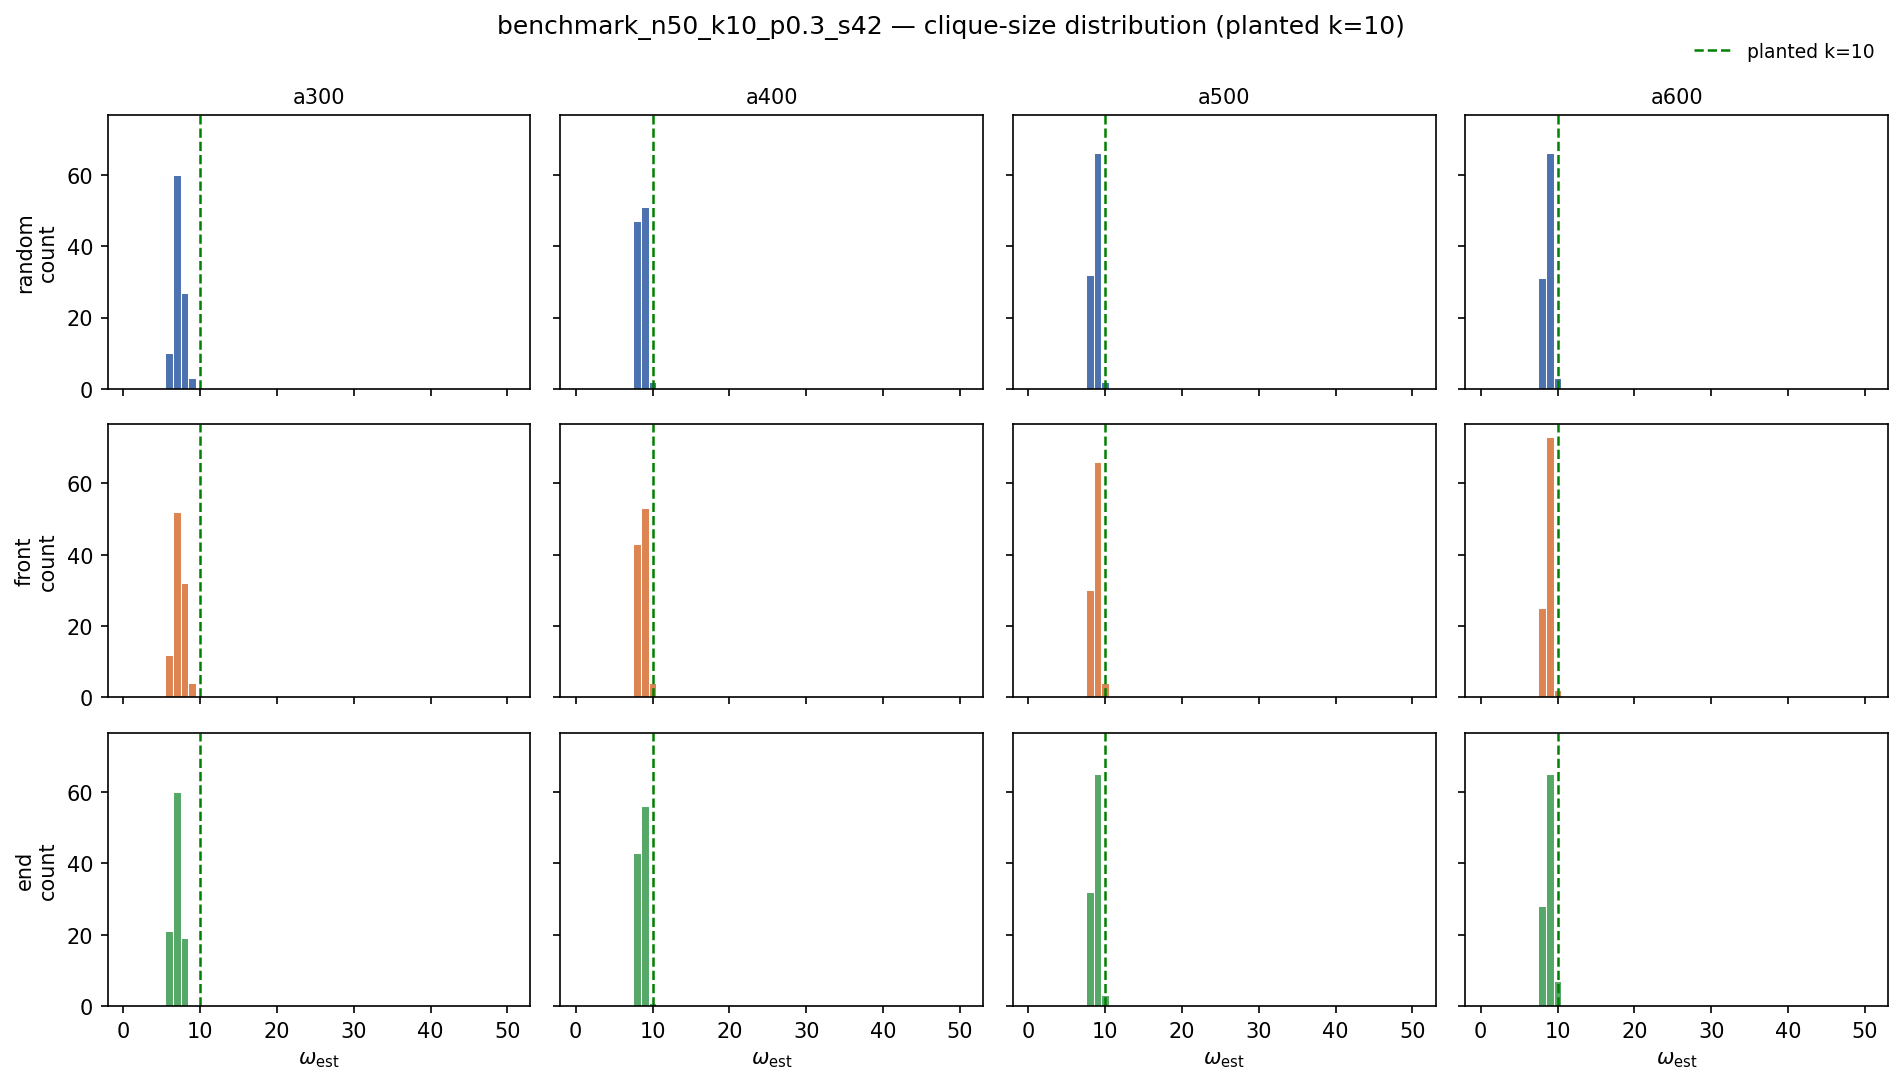
\includegraphics[width=0.48\linewidth]{benchmark_n50_k10_p0.3_s42/hist_omega_benchmark_n50_k10_p0.3_s42.png}\hfill
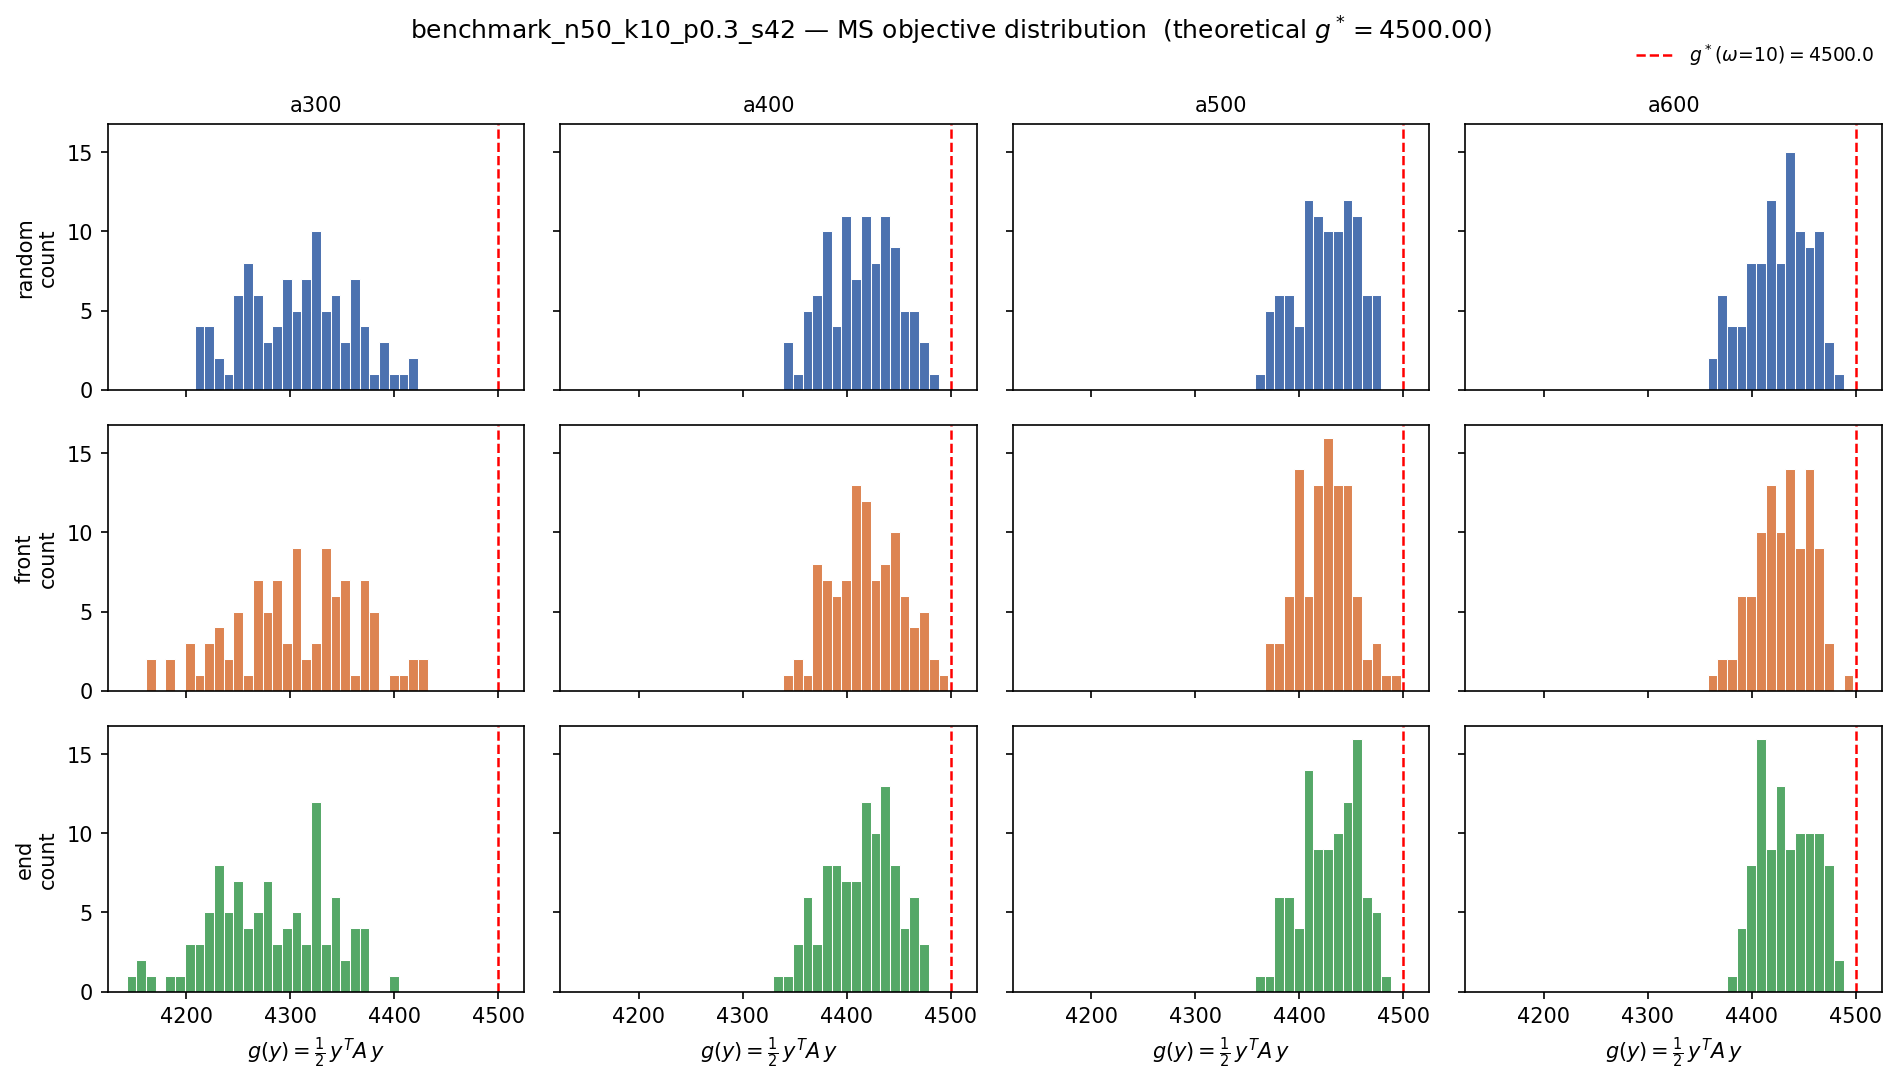
\includegraphics[width=0.48\linewidth]{benchmark_n50_k10_p0.3_s42/hist_objective_benchmark_n50_k10_p0.3_s42.png}\\
\footnotesize
Left: $\omega_{\mathrm{est}}$ mass concentrates at $9$ even though best
$g$ is within $0.15\%$ of $g^\ast(k{=}10)$. Right: objective distribution
shifts towards $g^\ast$ as amplitude rises.
\end{frame}

\begin{frame}{Appendix: \texttt{n100\_k22} — clique-size and objective grids}
\centering
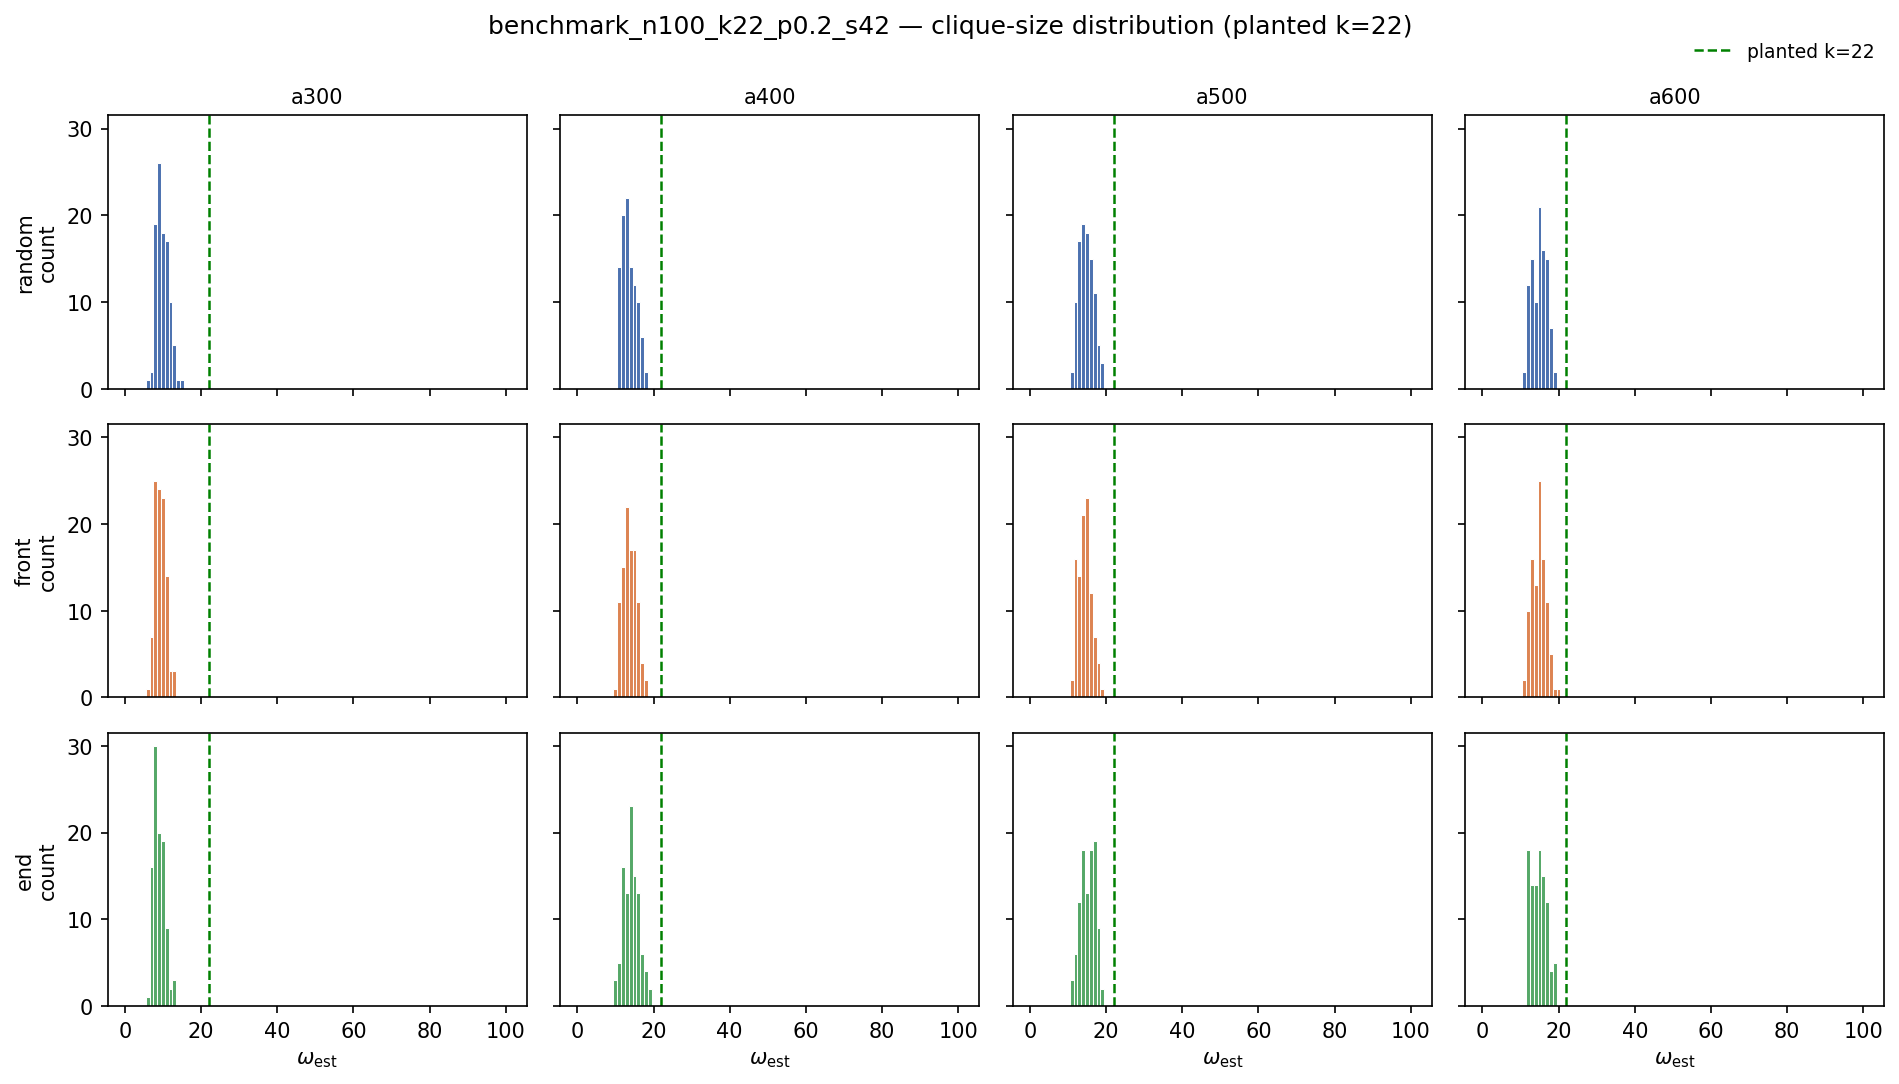
\includegraphics[width=0.48\linewidth]{benchmark_n100_k22_p0.2_s42/hist_omega_benchmark_n100_k22_p0.2_s42.png}\hfill
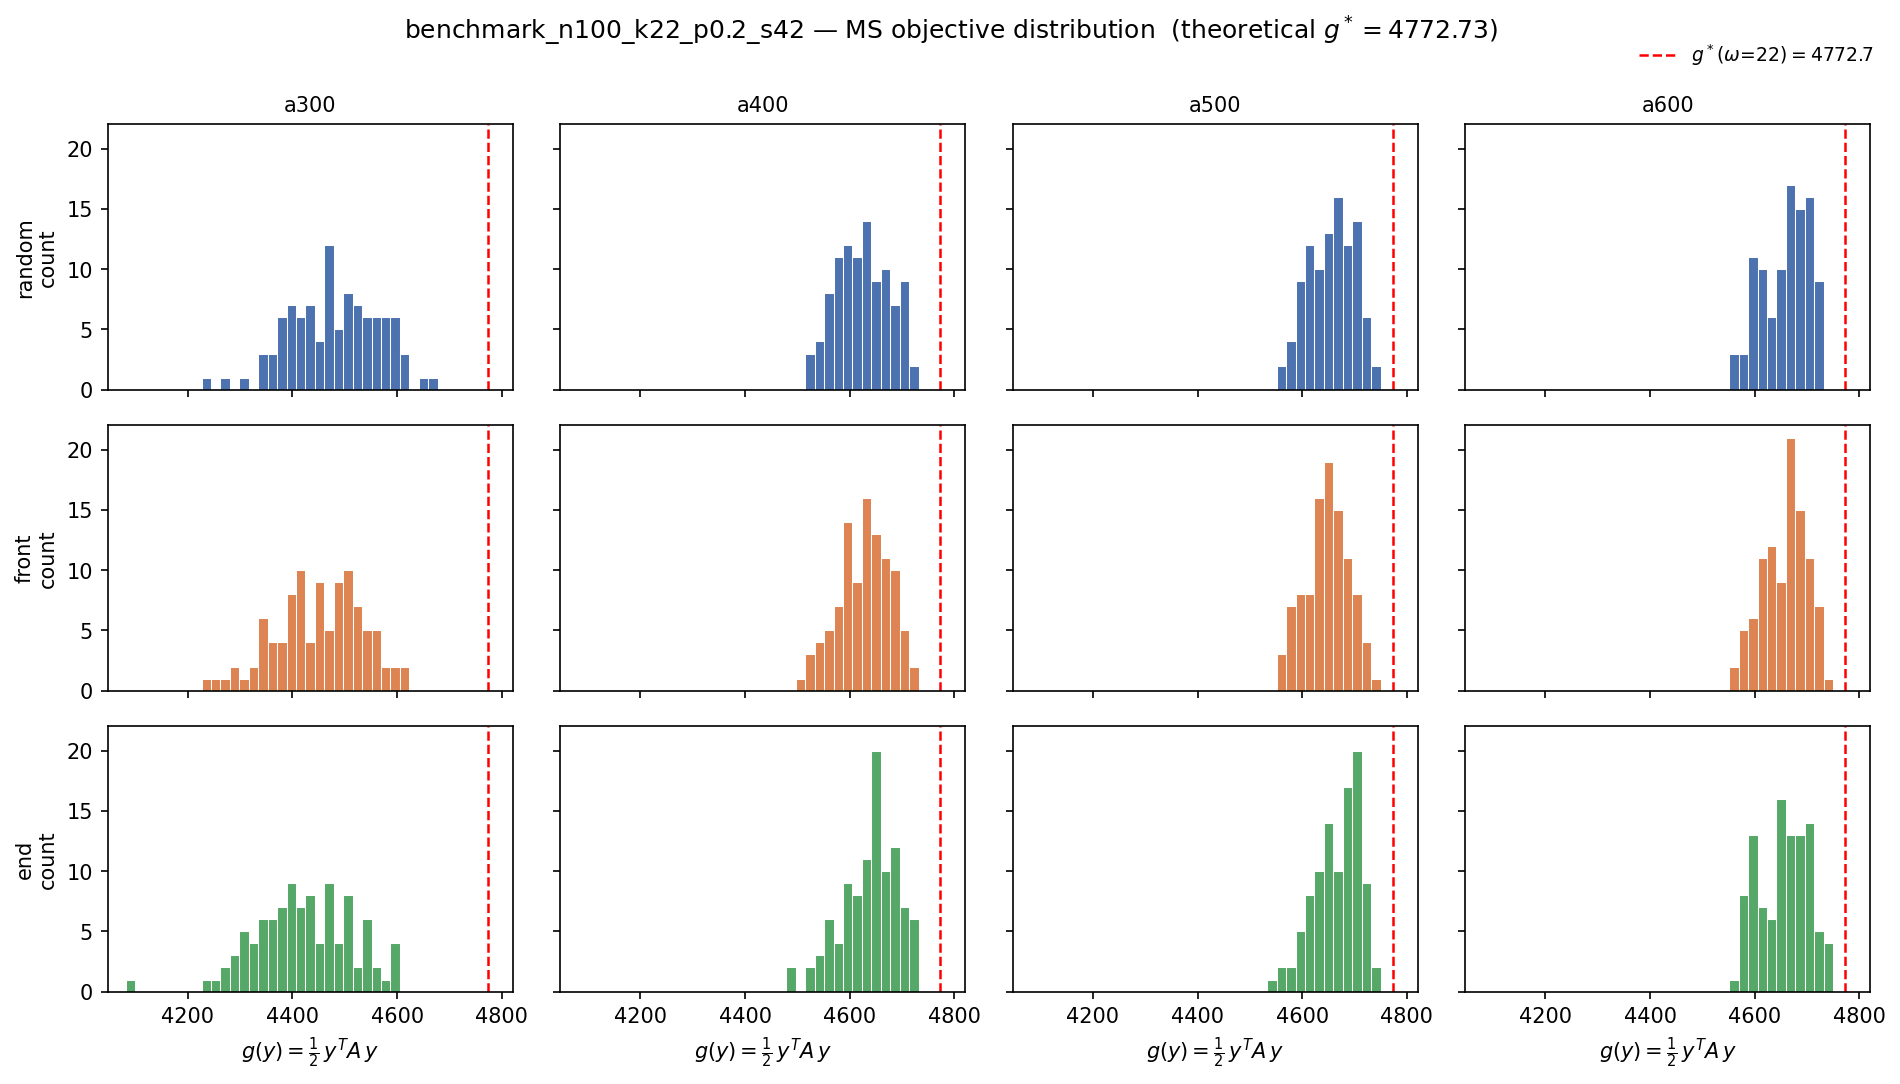
\includegraphics[width=0.48\linewidth]{benchmark_n100_k22_p0.2_s42/hist_objective_benchmark_n100_k22_p0.2_s42.png}\\
\footnotesize
Larger instance: $\omega_{\mathrm{est}}$ spreads over $17$--$21$; objective
distributions still tight and consistent across variants.
\end{frame}

\end{document}
